\documentclass[11pt]{article}   % Mandatory
\usepackage[T1]{fontenc}        % Support for fonts with æøå and other foreign characters.
\usepackage[utf8]{inputenc}     % Support for UTF-8 encoded input documents
\usepackage{fullpage}
\usepackage{graphicx}           % Support for including graphics as png, gif, and jpeg
\usepackage{amssymb}            % Support for alterantive symbols
\usepackage{amsmath}            % Support for mathematical symbols
\usepackage{listliketab}        % Support for tabulated lists
\usepackage{enumitem}           % Support for indented description items and more
\usepackage[parfill]{parskip}   % Support for American style paragraphs
\usepackage{color}              % Support for colored text
%\usepackage{listings}           % Support for code listings
\usepackage{nameref}            % Enables refernces to names.
\usepackage{makeidx}            % For creating indexes
\usepackage{wasysym}            % For symbols as \smiley
\usepackage{hyperref}        	% For using URLs
\usepackage{utility/petri}      % For doing petrinet vector graphics
\usepackage{xspace}             % For adding a space only when necessary. See ePNS command below.
\newcommand{\epns}{\textbf{Extended Petri net Simulator}\xspace}
\newcommand\writer[1]{\nobreak\begin{flushright}\small\textbf{Author: \large\textit{#1}}\end{flushright}}
\makeindex

\def\signed #1{{\leavevmode\unskip\nobreak\hfil\penalty50\hskip2em
  \hbox{}\nobreak\hfil(#1)%
  \parfillskip=0pt \finalhyphendemerits=0 \endgraf}}

\newsavebox\mybox
\newenvironment{aquote}[1]
  {\savebox\mybox{#1}\begin{quotation}}
  {\signed{\usebox\mybox}\end{quotation}}

\title{Project Definition\\ \epns}
\author{Group A}
\date{\today}

\begin{document}
\maketitle

\begin{abstract}
This paper is a definition to our Software Engineering 2 project. It will provide an outline of our project, while also introducing concepts and terms going to be used in our Systems Specifications.
\end{abstract}

\tableofcontents \newpage

\section{Introduction}
\writer{Thibaud, Albert}

\begin{quotation}
Petri nets, as graphical and mathematical tools, provide a uniform environment for modelling, formal analysis, and design of discrete event systems. \footnote{Petri Nets and Industrial Applications: A Tutorial. Richard Zurawski, MengChu Zhou.}
\end{quotation}

Petri nets are used as a means to model systems, but, as they are a mathematical concept, they are not always easy to understand for the ordinary user. Complex systems can be modelled with Petri nets, and usually, this would be an engineer's job. Even though engineers can easily create and understand their own Petri nets, every team member in a company would like to be able to understand what a Petri net is about without having any knowledge of the concepts behind them.

Therefore, the project aims at creating a 3D visualisation from a Petri net, to allow non-Petri net experts to actually to understand how the model works and validate a system.

However, Petri nets were not intended to have a 3D representation. For instance, there is no graphical concept or way to say that a particular Petri net would look like a train track because it was used to model a railway system. 

Thus, our goal for this project is the following: Providing an extension to Petri net models to make their 3D visualisation possible. For this purpose, we have imagined a simple link between a Petri net and a 3D visualisation.

\subsection{Conventions}

The priority of the requirements in Section \ref{sec:system-features} and \ref{sec:non-functional} will be indicated by the keywords \textbf{shall}, \textbf{should} and \textbf{would be nice}:

\begin{itemize}
	\item \textbf{Shall}: Requirements that must be implemented as a minimum, resources must be allocated to these requirements.
	\item \textbf{Should}: Requirements that add more functionality to the software, but are not the core required to work, if possible, resources will be allocated.
	\item \textbf{Would be nice}: Requirements considered good ideas and would be implemented if there are sufficient resources or in later versions of the software.
\end{itemize}

\subsection{Audience}

The audience of this document are persons affiliated with the company that models and simulates Petri net, developers of the system and final users of the Extended Petri net Simulator.
\section{Overall description}
\label{sec:overall}
This section describes the software and provides a brief explanation on how the system works.

\subsection{What are Petri nets?}

Petri nets are a graphical and mathematical modelling tool for describing concurrent and distributed systems. Some examples of their applications are work flow management, embedded systems or traffic control. The main advantages of Petri nets are their graphical notation, their simplicity on the semantics, and their rich theory for analysing their behaviour. However, using the Petri net graphical notation for understanding a complex system is quite hard, and thus a user-oriented visualization is required in a way that can be understandable to users which are not necessarily familiar with Petri nets.


\begin{figure}[htp]
\begin{center}
  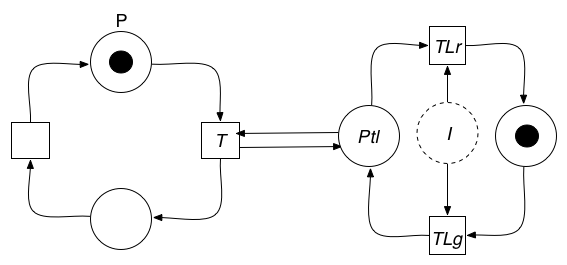
\includegraphics[width=0.8\textwidth]{image/petrinet_diagram.png}
  \caption{An example of a basic Petri net}
  \label{fig:petrinet}
\end{center}
\end{figure}

Figure \ref{fig:petrinet} presents an example of a basic Petri net. There are four different elements:

\begin{itemize}
\item Places: signified by circles, represent states.
\item Transitions: signified by squares, represent conditions.
\item Arcs: indicate which places are preconditions/postconditions for which transitions.
\item Tokens: signified by the dots, represent the elements that move in the Petri net along the places through the transitions.
\end{itemize}


Furthermore, we can see the example of \ref{fig:petrinet} as a model for a railway with a traffic light. The token in Place P represents a train moving on a railway. When this train arrives to Place P, the transition T will fire if the conditions are met. The only condition for a transition to be fired is that a token should be present on each of the incoming places of the transition.

In this scenario, the conditions are not met, as the required token in Place Ptl is missing. The visualization of this scenario would be a traffic light with a red light. If a user clicks on the Place I, it would generate a token that will turn the traffic light to green and thus the train will move.

With the aim of creating a visualization of the scenarios for the above Petri net model, an application tool is needed in order to allow the user to define where each of the elements are represented in the 3D world (geometry editor) as well as how these elements are represented (shape) and how they behave (animation). 

\subsection{Adding geometry to Petri nets}
The problem this project is tackled with is simple: We need a way to link the Petri net model to a 3D visualisation. For this purpose, once a Petri net model is created and its real life design is well-designed in the user's mind, what we call a "Geometry" is created.

For this purpose, there is a need of a geometry editor which will be used to assign a two dimensional location to the elements defined in the Petri net.

\subsection{Adding appearance to Petri net objects}
\label{sec:appearance}

Once the geometry problem is solved, a shape for each object should be defined. For instance, if places represent tracks, the shape, texture and other attributes should be linked to that object.

For this purpose, there is a need of an appearance editor which will be used to assign 3D visualization features to the elements defined in the Petri net.

\subsection{Configuration}

Before running the simulation, a definition of how the previous models are connected is needed. This is done in the configuration step as well as the validity check for the Petri net's connections to the geometry. 

\subsection{Simulating Petri nets}
The next step in visualizing Petri nets is add descriptive visuals. With the information provided by the Petri net, geometry and appearance as defined in the configuration file, the simulation is set up.

\begin{figure}[htp]
\begin{center}
  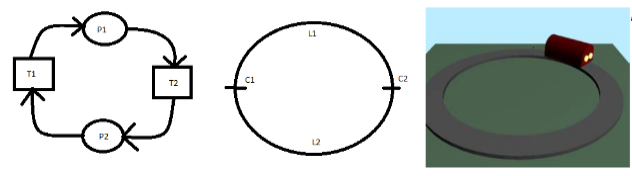
\includegraphics[width=0.8\textwidth]{image/3steps.png}
  \caption{Left: a simple Petri net.  Center: a geometry model. Right: A 3D visualization.}
  \label{fig:3steps}
\end{center}
\end{figure}

Using 3D models, textures and animations, the Petri net becomes easier to understand for the user. Continuing with the railway example, tokens become trains that move on tracks, which are places. As the tokens move from place to place, the train is animated in the 3D visualization along the tracks.

Figure \ref{fig:3steps}  shows how a simple 3D simulation of a train track and a train is made out of Petri net model and a simple geometry. Place P1 references L1 as its geometry and also has the shape of a track. The token on place P1 has the shape of a train and it moves with an animation defined by the place P1.
\section{Functionality}

In order to implement the functionalities of the concepts described in the previous section, editors are needed. Each of these editors will be described in this section.

\subsection{Petri net Editor}

\subsubsection{Purpose}
The basis for the main functionality of the software is the Petri net Editor. This editor enables a user to create or edit a Petri net that can be interpreted and used by the other editors. 

\subsubsection{Users}
Users with knowledge of Petri net logic and general technical skills are the main users of the Petri net editor. However, both simple and complex Petri nets can be implemented, so the technical skills of the users may vary accordingly. 


\subsubsection{Use cases}
The main use cases of the Petri net Editor are conveyed in the following diagram:

\begin{figure}[htp]
\begin{center}
  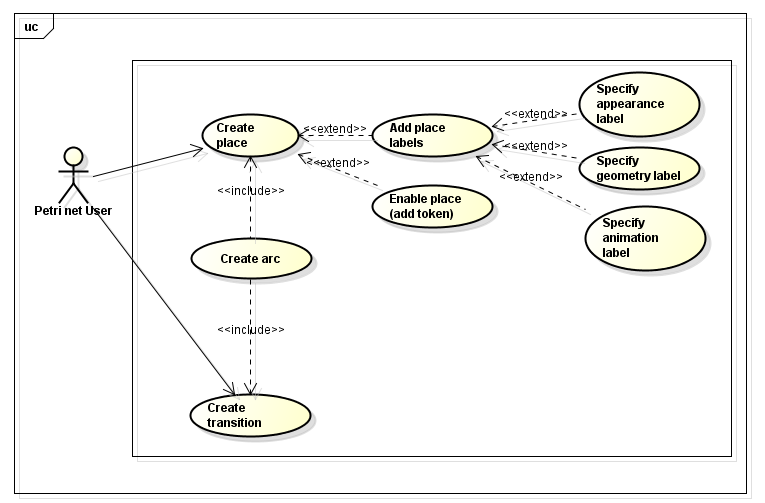
\includegraphics[width=0.8\textwidth]{image/PetrinetUC.png}
  \caption{Use cases for the Petri net Editor}
  \label{fig:petrinet_editor_usecases}
\end{center}
\end{figure}


The user will be able to create places, arcs and transitions. The user must start by creating a place or transition, arcs can only be created once there is a target and a source. A place or a transition can be dragged from a menu to the canvas, while the arc must be selected in the menu, then dragged from the source to the target. The user will be able to make the arc bi-directional by dragging a new arc in the opposite direction of the existing. 

A place can have up to three labels associated: appearance, geometry and animation. These labels are used to control the appearance, geometry and animation in the simulator. 

An example of an appearance label is "train", which will tell the simulator to use the appearance linked to "train" for the token(s) and the arcs associated with the place. See "Appearance editor" Section \ref{sec:appearance}. An example of an animation label is "fast", which will enable a fast token movement on the place and associated arcs. An example of a geometry label is "line\_1", which will link the place to a line specified in the geometry editor. 

Finally, a user can enable a place to receive input during runtime; this will enable the user to add a token on that place.

The Petri net editor is linked to the other editors, especially through labels. In the following, the Geometry editor will be described. 

\subsection{Geometry editor}


\subsubsection{Purpose}
As it has been previously discussed in Section \ref{sec:overall}, in order to create a 3D representation of the Petri net model, we need to add some geometrical information to it.  For this purpose, the user will interact with a geometry editor to define the location of the objects defined by the Petri net editor. These objects on their location will later be displayed in the 3D visualisation model. 
The geometry editor will allow the user to:
\begin{itemize}
\item draw lines - corresponding to places in the Petri net model
\item add bend points to lines - for creating curved lines
\item draw connectors - corresponding to transitions in the Petri net model
\item add input points  - corresponding to special constraints for transitions (e.g switches, traffic lights, etc.)
\end{itemize}

\subsubsection{Users}
The geometry editor will be used by technical users who are familiar with basic geometrical concepts and have a clear vision on how a geometry model is designed. No other specific previous knowledge is required but comprehension of Petri net models is an advantage.
\subsubsection{Use cases}
The main use cases of the Geometry editor are displayed in the following diagram:

\begin{figure}[htp]
\begin{center}
  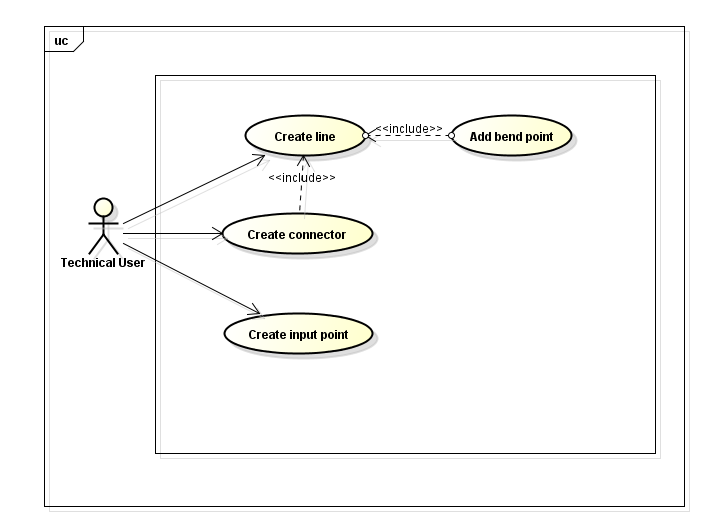
\includegraphics[width=0.8\textwidth]{image/GeometryUC.png}
  \caption{Use cases for the Geometry Editor}
  \label{fig:geometry_editor_usecases}
\end{center}
\end{figure}

\begin{enumerate}
	\item \textbf{Create line}: The user drags a line from the editor menu and draws it in the canvas. The number of lines is not restricted so the action can be repeated as many times as it is necessary but it is compulsory to have two connectors created before attempting to draw a line. Lines should also have a label that links back to the Petri net element it refers to.
	\item \textbf{Add bend point}: Bend points can only be added after a line has been created by clicking the line in order to create a curve. The number of bend points per line is restricted to one.
\item \textbf{Create connector}: Connectors can also be created from the editor menu and drawn in the editor window. Their functionality is to link two or more lines together. 
\item \textbf{Create input point}: Input points will be created in a similar way from the editor menu and can be placed anywhere in the canvas. However, they will have a label and an appearance attached to them in order to define the link back to the Petri net.   
\end{enumerate}

\subsection{Appearance Editor}
\subsubsection{Purpose}
The next step in reaching the 3D visualization of the Petri net model is to determine the visual characteristics for each element in the model. For this purpose, the appearance editor is used to define the shape, color, texture and any other information needed for a clear display of the initial model. 
\subsubsection{Users}
	The appearance editor can be used by any user both technical and nontechnical as it only implies linking the appearance labels defined in the Petri net model to a file containing all the information related to visual aspects: shape, texture, color. These can be .jpg files or special 3D documents whose structure is yet to be discussed.

\subsubsection{Use cases}
	The main use cases of the appearance editor are conveyed in the following diagram: 
	
	\begin{figure}[htp]
\begin{center}
  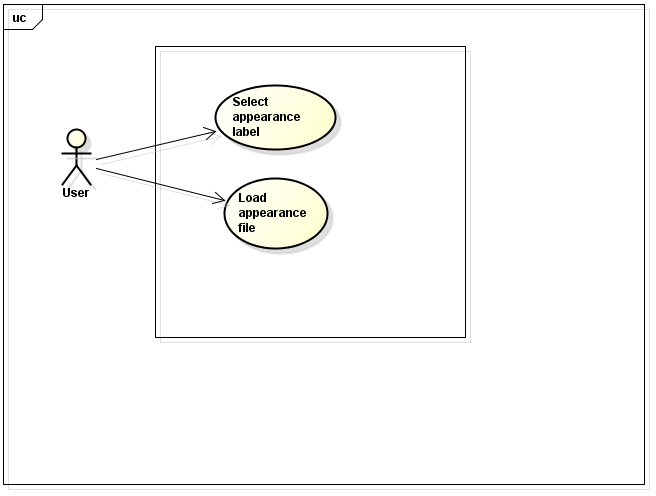
\includegraphics[width=0.8\textwidth]{image/AppearanceUC.png}
  \caption{Use cases for the Appearance Editor}
  \label{fig:appearance_editor_usecases}
\end{center}
\end{figure}


%\subsection{Use case description}

\begin{enumerate}
\item \textbf{Select appearance label}: The user will be able to select one of the appearance labels previously defined in the Petri net editor from a pop-up menu. For example, if the user wants to add appearance information to a token which in the Petri net model has as appearance label "train", then his/her selection from the pop-up menu should also be "train". The next step is described in use case 2. 
\item \textbf{Load appearance file}: The appearance editor will allow the user to browse among a list of files containing information related to the 3D visualization and load the one corresponding to the previously selected label.  
\end{enumerate}

   
 
\subsection{Configuration Editor}
\subsubsection{Purpose}
The configuration editor is intended to define a link between the Petri net model, the geometry and the appearance information files previously created by the user. Each element in the Petri net should have a corresponding geometry figure and appearance features assigned in order to have a valid configuration file for the simulation.   
\subsubsection{Users}
This editor will be used by all users, both technical and nontechnical as it only implies the association between three existing files. The interface should be intuitive and organised in a way that is familiar to the user in terms of loading files therefore no particular knowledge is required. 
\subsubsection{Use cases}
The main use cases for the configuration editor are conveyed in the following diagram: 

\begin{figure}[htp]
\begin{center}
  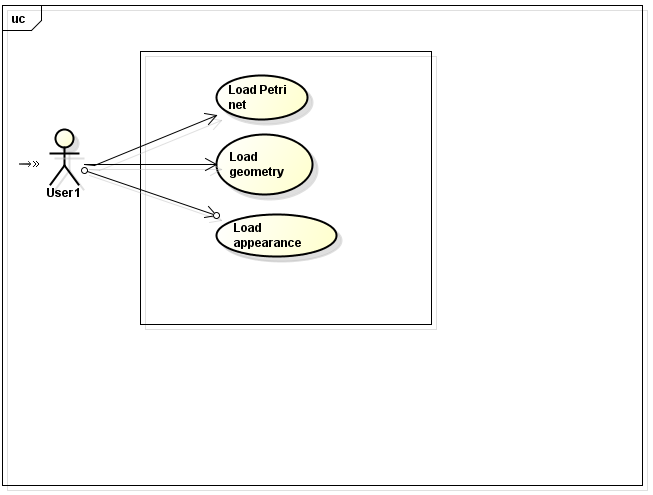
\includegraphics[width=0.6\textwidth]{image/ConfigurationUC.png}
  \caption{Use cases for the Configuration Editor}
  \label{fig:configuration_editor_usecases}
\end{center}
\end{figure}

\begin{enumerate}
\item \textbf{Load Petri net}: The user will be able to browse and load a Petri net model file designed using the Petri net Editor.
\item \textbf{Load geometry}: The user will be able to browse and load a geometry file designed using the Geometry Editor.
\item \textbf{Load appearance}: The user will be able to browse and load an appearance file designed using the Appearance Editor.
\end{enumerate}

\subsection{Simulator}
\subsubsection{Purpose}
Once the Petri net Editor and Geometry Editor have been set up correctly the user will be able to run the 3D simulation based on the information from the Appearance and Geometry Editor. During the 3D simulation the user will be able to add or remove trains, control traffic lights and control railroad switches through a Graphical User Interface (GUI).
\subsubsection{Users}
The simulator can be used by any user, both technical and nontechnical as they both have an interest in seeing the 3D visualization of the work done in the editors. Users do not need to have any prior knowledge about Petri nets since the simulation is controlled with a GUI and has no visual connection to the Petri net. 
\subsubsection{Use cases}
The main use cases for the Simulator are conveyed in the following diagram: 

\begin{figure}[htp]
\begin{center}
  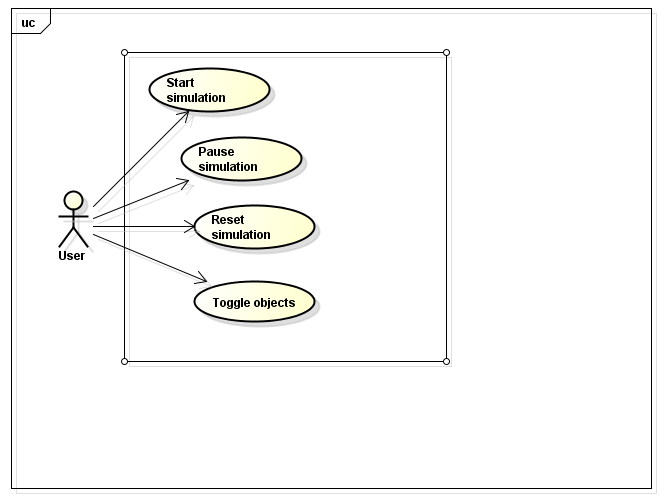
\includegraphics[width=0.8\textwidth]{image/SimulatorUC.png}
  \caption{Use cases for the Simulator}
  \label{fig:simulator_usecases}
\end{center}
\end{figure}

\begin{enumerate}
	\item \textbf{Start, pause and reset}: The user is able to start, pause and resume the simulation with 2 different buttons: one for play and pause, and another for resetting the simulation.
	
	\item \textbf{Toggle objects}: The user can toggle an object, for example a traffic light, in the simulation by clicking on it; switching (e.g.) a light from green to red or the other way around. 
\end{enumerate}





\section{Platform}

\subsection{Requirements}
The Petri net simulator runs with extensions in the Eclipse Kepler IDE , and is written in Java. The Eclipse platform is open source and free. Eclipse is cross-platform, and runs on Linux, Mac OS X, Solaris and Windows. 

Any modern PC should be able to run the Petri net simulator easily. The recommended minimum resolution is 1366x768 or equivalent. A mouse and keyboard is also recommended.
\section{Glossary}
\begin{description}

\item [3D] Three dimensional.

\item [Bendpoint] Bendpoint is a point, which functions as a control point for parametric curves allowing “bending” of said curve.

\item [Bézier-curve] Bézier-curve is a parametric curve, where shape is defined by blend of different control points.

\item [Catmull-rom] Catmull-rom splines are a family of cubic interpolating splines formulated such that tangent at each point of the spline is calculated using the previous and next point on the spline. (http://www.cs.cmu.edu/~462/projects/assn2/assn2/catmullRom.pdf)

\item [Connector]  Connector serves as either first or the last point of line.

\item [ePNK] Eclipse Petri Net Kernel.

\item [Geometry object] Geometry object can be either point or line.

\item [GUI] Graphical User Interface

\item [Input Point] Input Point is a point, where user is allowed to add tokens during the simulation.

\item [Javadoc standard] Format used by Javadoc is the industry standard for documenting Java classes.

\item [Parametric curve] Parametric curve is a mathematical curve defined by point locations.

\item [Petri net] A mathematical and graphical model for the description of distributed systems. It is a directed bipartite graph, in which nodes represent transitions and places. The directed arcs describe which places are pre- and/or post-conditions for which transitions. [source wiki]

\item [Point] Point is a coordinate location in a two dimensional plane.

\item [Token] Petri net element which moves along the Petri net places through transitions.

\item [UML] Unified Modeling Language - standardized, general-purpose modeling language in the field of software engineering. [source wiki]

\item [Use case] A list of steps defining interactions between a role (e.g. "technical user"), also known as an actor, and a system for achieving a goal. The actor can be a human or an external system.





 \end{description}

\printindex

\end{document}

